
\begin{savequote}[10pc]
\sffamily 
``\ldots the goal is to transform data into information and information
into insight.''
\qauthor{Carly Fiorina (1954--)}
\end{savequote}
\lstdefinelanguage{JavaScript}{
     keywords={attributes, for, class, classend, do, empty, endif, endwhile, fail, function, functionend, if, implements, in, inherit, inout, not, of, operations, out, return, set, then, types, while, use},
     comment=[l]{//}
}
\lstset{language=JavaScript}
\chapter{Main user interface}\label{chap:client}
Users are unlikely to appreciate the Web Services developed in the last
part. They merely serve data; that data needs processing and a proper
presentation in order to be converted to information relevant for the user. In
this chapter, we describe the design and implementation subtleties regarding the
main user interface of the mashup. The client is an Ajax client conveying surf
weather information that assist practitioners of wind sports.

\section{Design}
An overall requirement for the user interface is conveying relevant
information in a way that is easily comprehensible for the user. The key to
fulfill this requirement is 1) to present the information in a graphical way, and
2) to reduce the information to the relevant only in terms of the location of the
user. In essence, the main client is a geographical information system.

We embrace the requirements by a design consisting of three pages all visualizing
data on a map. The map is centered around the location of its user which filters
away most irrelevant information from the user interface. Surf spots are pivotal
in the application and are available on all pages. Weather observations and
weather forecasts are separated on two different pages due to their conceptual
difference. Otherwise, forecasts and observations are displayed in the same way:
an arrow in the wind direction and with a color indicating the speed. Spots are
shown on all maps with a green circle with a cross in it. Finally, we have a
page where spots are input or edited.

Figure~\ref{fig:ajax_ui} shows an early prototype of the user interface. The
current application still has a design consisting of three pages. Page 1,
however, shows an initial idea for visualizing: uniting spots and weather
data. There exists no guarantee for a weather station near spots, and forecasts are
conceptually inappropriate for flag illustration; therefore, spots and weather
data is kept separate in the current design. Page 2 shows the observations on a
map. Page 3 shows the page where users enter new spots in the application.

\begin{figure}[htbp]
  \centering
  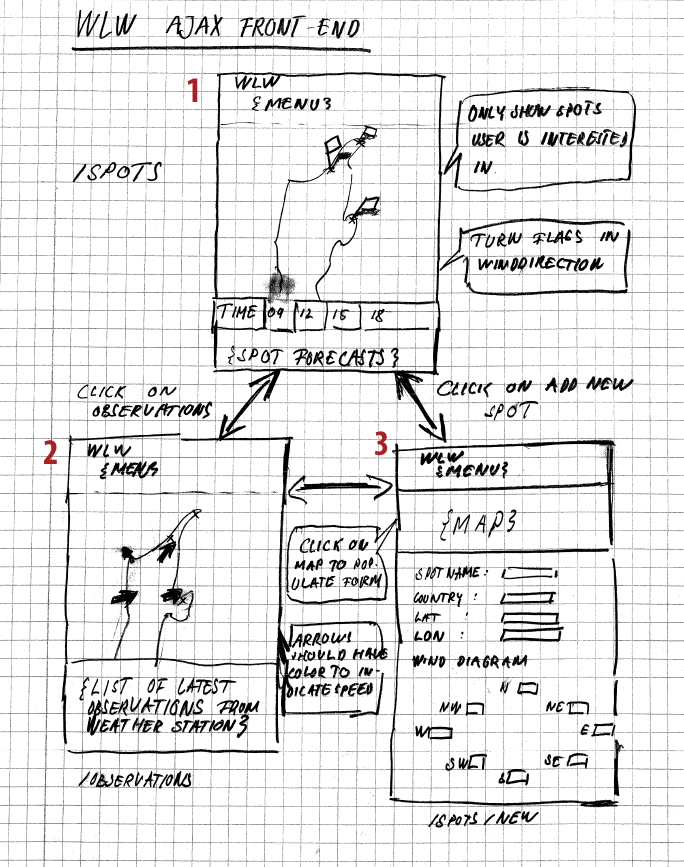
\includegraphics[width=\textwidth]{./Figures/ajax_ui}
  \caption{Paper prototype of main user interface} 
  \label{fig:ajax_ui}
\end{figure}

\section{Finding the location of the client}
A pivotal requirement for the weather service is delivering location-aware
geographic information. This demands that the location of the client is known.
Ideally, the user client tracks the user's location by any available means, e.g.,
IP-address, GPS, or GSM localization, sends the geographic information to the
server that responds with a resource representation relevant for the location. W3C is working
on the Geolocation API Specification that embrace the requirement
\citep{w3:geo_api}. The specification is novel but browsers vendors have begun
supporting it in their beta versions, e.g.,
Opera\footnote{\url{http://my.opera.com/core/blog/geolocation-enabled-build}} and
Mozilla\footnote{\url{https://developer.mozilla.org/En/Using_geolocation}}.

The API is obviously the future, however, the API is not yet supported to an
extent where we would consider using it. At the moment a more viable approach is
using the Google Gears Geolocation
API\footnote{\url{http://code.google.com/apis/gears/mobile.html}}, which among
others the W3C Geolocation API specification builds upon. Google Gears also
support mobile devices, however, only a handful.

JavaScript that use Google Gears triggers a popup in browsers. The popup ask
users to grant permission to the Web application in order to store information on
their computer. The popup is intimidating for users and a sole reason for
another solution.

\url{ipinfodb.com} is a free geolocation service. The service converts from IP
address -- uri-encoded in a GET request -- to a geographical position returned in
either XML or JSON(P). An example: a request such as
\begin{verbatim}
http://ipinfodb.com/ip_query.php?output=json&callback=foo
\end{verbatim}
returns a JSON object wrapped in the \verb|foo| function indicating the
approximate location of the callers computer. Since the returned format is valid
JavaScript requests are directly loaded from the source into client, it just have
to be dynamically inserted into the \verb|<script>| tag. Luckily, jQuery
abstracts that away in the \verb|getJSON| function.

Listing~\ref{lst:iploc} shows how the We Love Wind client uses
\verb|ipinfodb|. The client avoids calling \verb|ipinfodb| repeatedly by storing
the result of the first request as a cookie that is valid for one day.\footnote{A
thorough introduction to cookies in JavaScript is available at
\url{http://www.quirksmode.org/js/cookies.html}} \verb|getLocation| is the entry
function; when a location cookie is not present the client fetches its own
location from \verb|ipinfodb| using \verb|geoIP| and JSON(P).

\begin{lstlisting}[caption=Tracking client location with ipinfodb and JSONP, label=lst:iploc]
// get the lat/lon of this user ip address
function geoIP(callback){
    jQuery.getJSON("http://ipinfodb.com/ip_query.php?output=json&callback=?", function(data){
        var lat = data.Latitude;
        var lon = data.Longitude;
        callback({
            'lat': lat,
            'lon': lon
        });
    });
}

// get the lat/lng of the client
// if location cookie is set get this
function getLocation(callback){
    var location = readCookie('location');
    if (location) {
        var latlng = location.split(',');
        callback({
            'lat': latlng[0],
            'lon': latlng[1]
        });
    }
    else {
        geoIP(function(obj){
            createCookie('location', obj.lat + ',' + obj.lon, 1); // 1 day
            callback(obj);
        });
    }
}
// set location cookie
function setLocation(point) {
	createCookie('location', point.lat + ',' + point.lon, 1);
}  
\end{lstlisting}

\section{Reducing the data set}
The size of the application's data set that the client downloads will eventually
reach a significant size. A size that will hurt the client in terms of increased
latency and poor performance. The geohash grid is a natural means to reduce the
data set. We decrease the amount of data to download by reducing data to
geographical points that are in the neighbors geohash
area. Figure~\ref{fig:geohash_demo} shows the concept; only points within the
boxes are downloaded.


\begin{figure}[htbp]
  \centering
  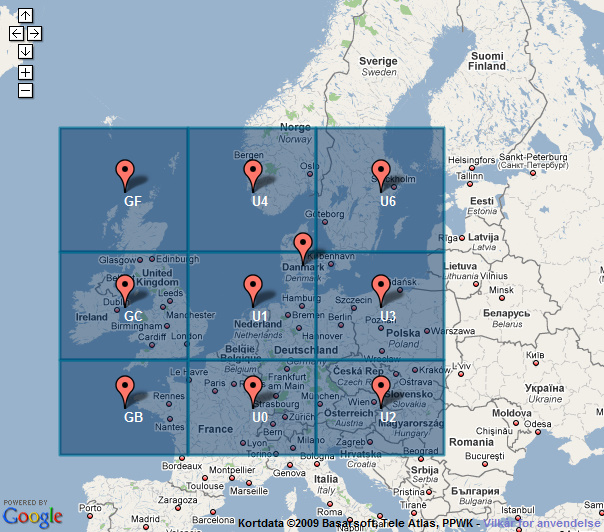
\includegraphics[width=\textwidth]{./Figures/geohash_demo}
  \caption{Geohash grid}
  \label{fig:geohash_demo}
\end{figure}  


The Web Service already supports geohash queries. However, the approach demands
that geohash encoding and grid neighbor finding is also in place at the
client. \citep{geohash:neighbors} is an open source geohash and grid neighbor
finding implementation. We have made the implementation compatible with most
browsers (removing non-standard ECMAscript) and added logic to handle case three
of navigating to neighbors (see Section~\ref{sec:lost}) and included it in the
client.

With geohash in place the client needs a transparent way of handling 1)
downloading points of different types: spots, weather stations, and forecasts
points, and 2) panning of the map which should trigger download of data from
untouched grid boxes. 

The two requirements is accomplished with the publish-subscribe pattern
\citep{Gamma:1995}. A geohash publisher is connected to the map subscribing to
map movement finished events. Upon such events the geohash publisher encodes
the geohash value of the new center, calculates all the neighbors, and publishes
all new geohashes to the subscribers.

We encourage the reader to access
\url{http://www.welovewind.com/examples/geohash/index.html} for a demonstration
of the concept.

\section{Seamless points loading}
With the geohash publisher in place we turn to the problem of seamlessly
downloading points in the published geohash grid cells and displaying the
downloaded points on the map. 

\begin{figure}[htbp]
  \centering
  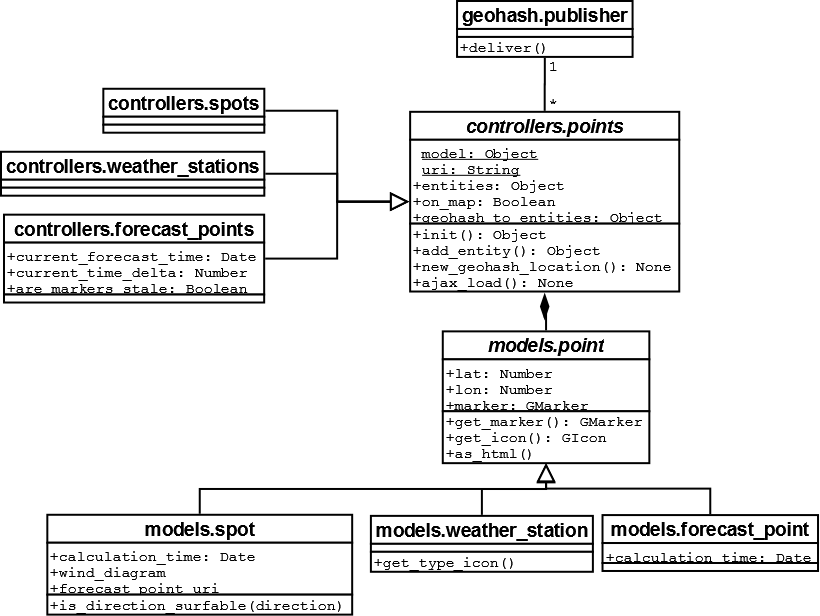
\includegraphics[width=\textwidth]{./Figures/js_model}
  \caption{Client architecture view (UML static structure diagram)}
  \label{fig:js_arch}
\end{figure}

All active geographical points are handled by a points controller, shown in
Figure~\ref{fig:js_arch}. The points controller contains logic to retrieve points
from the server given a geohash. In addition, other objects (not included in the
figure) can subscribe to the points controller, in which case the controller
delivers downloaded points to them. The application currently has three
different types of points: spots, weather stations, and forecast points that all
inherit from the points controller. The ``subclass'' defines the URI of the
concrete Web Service resource, and defines the model for the concrete objects in
the JSON items list (present in all JSON list resources). The model is used to
augment the loaded JSON objects with logic, e.g, to display themselves on a map,
and determine the surfable direction of a spot.

An example of a subscriber of the points controllers is the map controller. The
map controller's responsibility is showing / removing categories of markers on
the map. Figure~\ref{fig:points_loading} shows the runtime architecture of points
loading, and their display on the map. First, all the publish-subscribe
relationships are setup. In addition, a map movement finished subscriber is setup
in the geohash publisher; the subscriber is the source that starts the following process:
\begin{enumerate}
  \item Upon a map movement finished event the geohash for the center of the map
is calculated.
  \item The neighbors are found and subscribers (the points controllers) are
delivered all new touched geohash grid cells.
  \item The points controllers then contact the server for points in the geohash
  cells.
  \item Upon return the points are de-serialized and augmented with logic. The augmented points are delivered
  to the subscribers, in this case, the map controller. 
  \item The map controller adds the points to the map.
\end{enumerate}

The architecture decouples objects and separates concerns. An advantage is that
any other controller interested in points can just add itself as a subscriber to
the different type of points it is interested in. 

\begin{figure}[htbp]
  \centering
  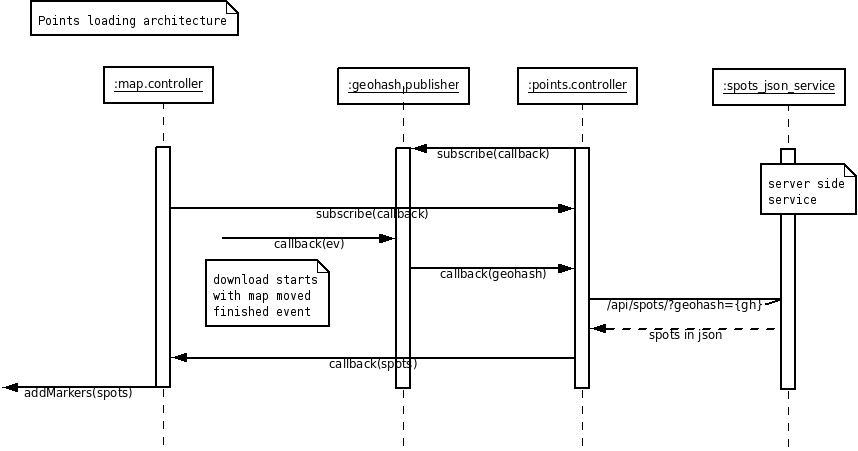
\includegraphics[width=15cm]{./Figures/arch_ajax_points}
  \caption{Points loading architecture view (UML sequence diagram)}
  \label{fig:points_loading}
\end{figure}

\section{Coordination between Ajax calls}
A requirement for the application is visualizing relevant forecasts coupled to
the surfability of spots. We have come up with a graph to visualize the current
and future surfability of spots, shown in Figure~\ref{fig:graph}.\footnote{The
graph is created with the open source jQuery-based graph tool flot:\\
\url{http://code.google.com/p/flot/}} An upward bar in the figure indicates that
the wind is in the correct direction (input by the users), and downward direction
means the wind is in the wrong direction. The colors correspond to the color map
in Figure~\vref{fig:frv}, except that when the wind direction is unsuitable the
color is black.

\begin{figure}[htbp]
  \centering
  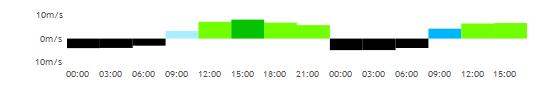
\includegraphics[width=\textwidth]{./Figures/graph}
  \caption{Surfability graph}
  \label{fig:graph}
\end{figure}

The graph demands the presence of both the spot and its corresponding forecast
point. With Ajax the ordering of returned calls is arbitrary. Thus, the client
should somehow coordinate the dependent requests and first when both points are
loaded create the graph.

Every points controller maintain a map from geohash to concrete point
entities. Whenever points from a new geohash are loaded they are inserted into
the map. When controllers subscribe to a points controller they specify a
list of dependencies in the form of references to other points controllers. When
points controllers publish updates to its subscribers the dependencies are
first checked and only if all have downloaded points from the geohash the
callback is triggered. Listing~\ref{lst:points.publish} shows the \verb|publish|
function in the common points controller that handles dependencies.

\begin{lstlisting}[caption=Dependency aware publish function,label=lst:points.publish]
// publish new points loaded
// Args:
//    geohash_prefix: geohash prefix of loaded models
points.publish = function(geohash, the_points){
  // publish points to subscribers
  subscribers_loop: for (var i = 0; i < points.subscribers.length; i++) {
    // check if dependencies are loaded
    for (var j = 0; j < points.subscribers[i].dependencies.length; j++) {
      var controller = points.subscribers[i].dependencies[j];
        
      // if other not loaded continue with next subscriber
      if (!controller.geohash_to_entities[geohash]) {
        continue subscribers_loop;
      }
    }
    // callback(points)
    points.subscribers[i].callback({
      'geohash': geohash,
      'points': the_points
    });
  }
}
\end{lstlisting}

\section{Drawing a circle with Google Maps}
The user interface creates surfability graphs for spots within a certain radius
of the user's location. The user interface needs some component
that indicates this radius to the user and let them adjust it. We apply a
circle as the means to indicate to users the radius of graph creation.

The Google Maps API provides no built-in functionality to draw circles on a
sphere. The API provides a \verb|GPolygon| that can be used to create arbitrary
geometry. There are examples of how to create a circle out of
polygons\footnote{Google Maps circle example:
\url{http://maps.forum.nu/gm_sensitive_circle2.html}}, however, none derive nor
explain the theory of the circle creation. In \citep{haver:veness} many
geographical information systems formulas for JavaScript are presented, however,
it contains no explanation. In the following, we derive the formula behind circle
creation.

\begin{figure}[htbp]
  \centering
  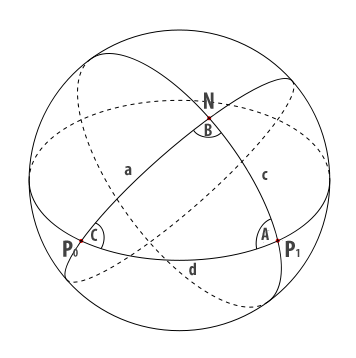
\includegraphics[width=8cm]{./Figures/circle_point}
  \caption{Spherical triangle on sphere} 
  \label{fig:sphere_distance}
\end{figure}

The first requirement is given a point, that will be the center of the circle,
find another point in a certain distance, and bearing from the center point. The
law of cosines, Theorem~\ref{thm:law_of_cosines}, can be used to find points in a
certain distance and bearing from another point. First we find the latitude of
that point.

\subsection*{Latitude}
Given the spherical triangle in Figure~\ref{fig:sphere_distance}, then 
\begin{equation}
  cos(c) = cos(a)cos(d) + sin(a)sin(d)cos(C) \tag{law of cosines}
\end{equation}
Let N be the North Pole, then the distances $a$ and $c$ is given by the
latitudes $P_0$ and $P_1$ respectively. Therefore,
\begin{equation}
  cos(\frac{\pi}{2} - P_{1_{lat}}) = cos(\frac{\pi}{2} - P_{0_{lat}})cos(d) + sin(\frac{\pi}{2} - P_{0_{lat}})sin(d)cos(C) \notag
\end{equation}
Since $cos(\frac{\pi}{2} - \phi) = sin(\phi)$,
\begin{equation}
  sin(P_{1_{lat}}) = cos(P_{0_{lat}})cos(d) + cos(P_{0_{lat}})sin(d)cos(C) \notag
\end{equation}
That is, given a point $P_0$, another point $P_1$ in bearing $C$ and distance $d$
from $P_0$, the latitude of the point $P_1$ is given by
\begin{equation}
  P_{1_{lat}} = asin(cos(P_{0_{lat}})cos(d) + cos(P_{0_{lat}})sin(d)cos(C)) \notag
\end{equation}

% http://en.wikipedia.org/wiki/Spherical_trigonometry
\subsection*{Longitude}
From the last subsection the latitude of the new point is now known. Given that
the angle $B$ on the figure is known, the longitude of the new point,
$P_{1_{lon}}$ is given by
\begin{equation} 
P_{1_{lon}} = P_{0_{lon}} + B \label{eq:longitude_circle}
\end{equation}
We now derive a formula for the angle $B$. Given the spherical triangle in
Figure~\ref{fig:sphere_distance}, then
\begin{equation}
cos(d) = cos(a)cos(c) + sin(a)sin(c)cos(B) \notag
\end{equation}
Let N be the North Pole, then the distances $a$ and $c$ is given by the latitudes
of $P_1$ and $P_0$ respectively. Since $cos(\frac{\pi}{2} - \phi) = sin(\phi)$,
\begin{equation}
cos(d) = sin(P_{0_{lat}})sin(P_{1_{lat}}) + cos(P_{0_{lat}})cos(P_{1_{lat}})cos(B) \notag
\end{equation}
Isolating $B$,
\begin{equation}
cos(B) = \frac{cos(d) - sin(P_{0_{lat}})sin(P_{1_{lat}})}{ cos(P_{0_{lat}})cos(P_{1_{lat}})} \notag
\end{equation}
\begin{equation}
B = acos(\frac{cos(d) - sin(P_{0_{lat}})sin(P_{1_{lat}})}{ cos(P_{0_{lat}})cos(P_{1_{lat}})}) \notag
\end{equation}
The value for $B$ can now be inserted in (\ref{eq:longitude_circle}). Since
$acos$ returns the value in $[0;\pi]$ we have to handle the case when the bearing
is above $\pi$. In that case,
\begin{equation} 
P_{1_{lon}} = P_{0_{lon}} - B
\end{equation}
%
The very observant reader might have noticed something peculiar: the formula
derived does not match with the formulas used in the referred examples and
\citep{haver:veness}. Deriving the formulas used in those are much more
complicated and since they lack explanation it remains uncertain why they did
it that way.

From a mathematical perspective an interesting point is that the whole
theory, both for the distance formulas and the circle formulas breaks
down when one of the points is the North Pole. In that case the
``triangle'' is a line. In practice, however, it is not a problem
since on Google Maps it is not possible to get a point at 90�
latitude. It returns ca. 89.6�.

\subsection*{JavaScript implementation}
With the formulas in place it is easy to implement the function that finds a new
point in a certain bearing and distance from an originating point,
Listing~\ref{lst:javascript_destination} shows how. The function directly
reflects the formulas; because of small rounding errors $cos(B)$ might be larger
than 1, in that case we set it to one to avoid invalid input to $acos$.

\begin{lstlisting}[label=lst:javascript_destination,caption=Finding a point in a certain bearing and distance with JavaScript]
// Calculate a new point in the given bearing and distance
// from the given point
// Args:
//     point: GLatLng to calculate from
//     bearing: bearing in radians  
//     distance: distance to point
function destination(point, bearing, distance){
    var R = 6367; // earth's mean radius in km
    var d = distance / R; // unit sphere distance
    var P0_lon = point.lngRadians();
    var P0_lat = point.latRadians();
    
    var P1_lat = Math.asin(
        Math.sin(P0_lat) * Math.cos(d) + 
        Math.cos(P0_lat) * Math.sin(d) * Math.cos(bearing)
    );
    
    var cos_B = (Math.cos(d) - Math.sin(P0_lat) * Math.sin(P1_lat)) / 
        (Math.cos(P0_lat) * Math.cos(P1_lat));
    
    // secure against rounding errors.
    if(cos_B >= 1){
      cos_B = 1;
    }
  
    if(bearing > Math.PI) {
      var P1_lon = P0_lon - Math.acos(cos_B);
    }else{
      var P1_lon = P0_lon + Math.acos(cos_B);
    }
    // convert to degrees
    P1_lat = P1_lat * (180 / Math.PI);
    P1_lon = P1_lon * (180 / Math.PI);
    return new GLatLng(P1_lat, P1_lon);
};
\end{lstlisting}
Creating the circle on Google Maps is done by iterating from $[0;2\pi]$ creating
a list of points around the center with \verb|destination| and connecting them in
a \verb|GPolygon|.

\section{Summary}
In this chapter we presented the design of the Ajax client and the main
subtleties in the implementation of the client. The subtleties included 1)
loading points on a proximity basis, 2) loading additional points as users pans a
Google Map, 3) coordination of points loading, and 4) drawing a circle with
Google Maps.
